% De la numérisation à l’annotation : l'automatisation du traitement des sources

\subsection{Chaîne de traitement des sources historiques}
    \subsubsection{Du manuscrit aux diagrammes : construction d'une chaîne de traitement pour les sources astronomiques}
	Du point de vue de l'utilisateur, la détection d'objet dans une source numérisée représente une unique étape : après envoi d'une numérisation de manuscrit ou d'imprimé dans l'application, celle-ci est retournée après un délai accompagnée d'annotations qui signalent les illustrations détectées. Cette fluidité dans l'expérience de l'utilisateur repose sur une chaîne de traitement automatique qui prépare les sources pour leur affichage dans l'application et pour le lancement de la détection d'objet sur les images. Ces traitements, invisibles du point de vue de l'utilisateur, sont variés, allant de la transformation du format des fichiers soumis, à l'envoi de ces données à des outils externes, tels que des \api, pour leur traitement par des algorithmes de vision artificielle.
	
	Les traitements appliqués aux sources envoyées à l'application par les chercheurs du projet \eida est constituée de cinq grandes étapes (fig. \ref{fig:detection_workflow}), qui représentent elles-mêmes divers traitements appliqués au fichier soumis initialement, transformé à chaque étape. 
	
	\begin{figure}[h]
		\centering
		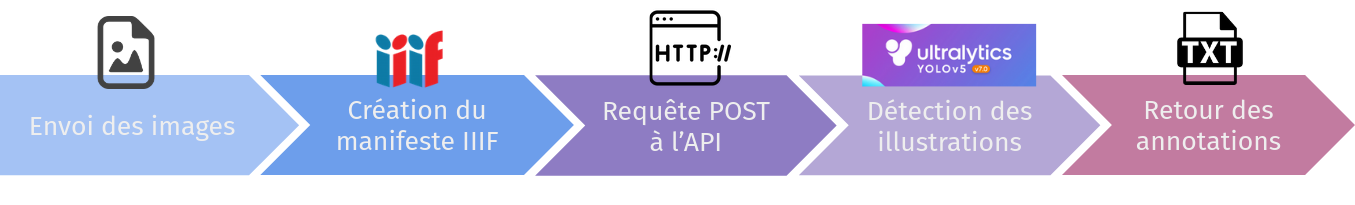
\includegraphics[width=16cm]{images/detection_workflow.png}
		\caption{Schéma de la chaîne de traitement du projet \eida pour la détection d'objet}
		\label{fig:detection_workflow}
	\end{figure}

	En premier lieu, depuis l'interface d'ajout d'un objet de l'application \eida (fig. \ref{fig:eida_list}), l'utilisateur remplit un formulaire de signalement du témoin avec un ensemble de métadonnées descriptives, et attache à ce formulaire une numérisation sous forme de manifeste \iiif, de fichier PDF ou d'un ensemble d'images aux formats \acrshort{jpeg} ou \acrshort{png}. Lorsque le formulaire est soumis, l'application retourne à l'utilisateur un message flash qui l'informe qu'un délai est nécessaire au traitement de la source, et que la numérisation annotée sera mise à disposition après finalisation de la détection. En parallèle, les images de la numérisation sont enregistrées : cette chaîne de traitement varie en fonction du format du fichier soumis par l'utilisateur\footnote{Les manifestes \iiif sont parsés pour en extraire les images, et les fichiers PDF sont fragmentés en une image par page et convertis en images au format PNG.}, et le résultat souhaité est l'enregistrement sur le serveur d'un fichier image par page de la numérisation.
	
	\begin{figure}[h]
		\centering
		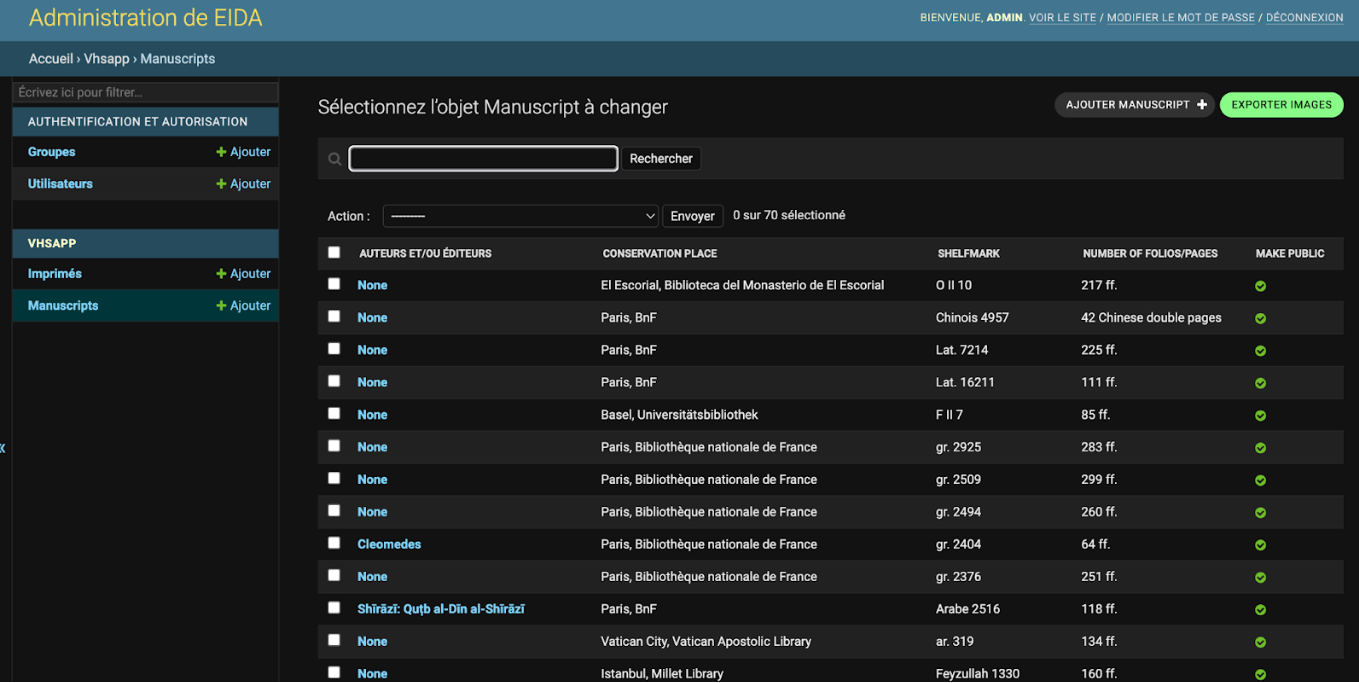
\includegraphics[width=16cm]{images/eida_list.png}
		\caption{Capture d'écran de l'interface listant les manuscrits saisis dans l'application \eida}
		\label{fig:eida_list}
	\end{figure}

	À partir des images de la numérisation enregistrées sur le serveur, un manifeste \iiif est généré par l'application\footnote{Comme mentionné dans la section \ref{stardardIiif}, malgré l'existence d'un standard, les manifestes \iiif présentent des disparités en fonction de leurs institutions d'origine. Pour assurer l'uniformité des manifestes utilisés pour la mise à disposition des sources du projet \eida, un nouveau manifeste est généré, y compris pour les numérisations déjà soumises sous la forme de manifestes \iiif.} : la numérisation est ainsi localisée par \URL, et peut être mise à disposition des utilisateurs selon un standard interopérable qui permet sa manipulation et sa réutilisation.
	
	Une fois le manifeste \iiif généré, une requête est envoyée à \exapi pour demander l'annotation des images par le modèle de détection. L'\URL du manifeste est envoyé par une requête \http POST : sa réception lance la chaîne de traitement des requêtes de l'\api, c'est-à-dire l'extraction et l'enregistrement des images à partir du manifeste \iiif, puis l'extraction des illustrations dans les images par le modèle de détection d'objet. 
	
	Après l'achèvement de la détection, le fichier d'annotations est retourné à l'application par une requête POST, et est enregistré sur le serveur. À partir de ce fichier texte, les détections sont indexées par le serveur \iiif d'annotation SimpleAnnotationServer\footcite{WelcomeSimpleAnnotation}, qui permet de lier les annotations avec les \textit{Canvases} correspondants dans une nouvelle version du manifeste \iiif du document étudié\footnote{Le manifeste \iiif de l'ouvrage existe donc en deux versions : une version \texttt{auto}, qui correspond à la numérisation sans annotations, et une version \texttt{v2}, à laquelle sont ajoutées les annotations.}. Cette indexation permet l'affichage des annotations sur l'image correspondante lorsque l'utilisateur consulte la numérisation dans un visualiseur \iiif.
	
	Le retour et l'indexation des annotations marque leur mise à disposition pour l'utilisateur : dans l'interface de modification des informations d'un témoin, un bouton permettant de visualiser les annotations apparaît (fig. \ref{fig:eida_buttons}), et permet de rediriger l'utlisateur vers une interface pour éditer manuellement les résultats de la détection automatique, et vers un visualiseur Mirador permettant de voir la numérisation accompagnée de ses annotations.	
	
	\begin{figure}[h]
		\centering
		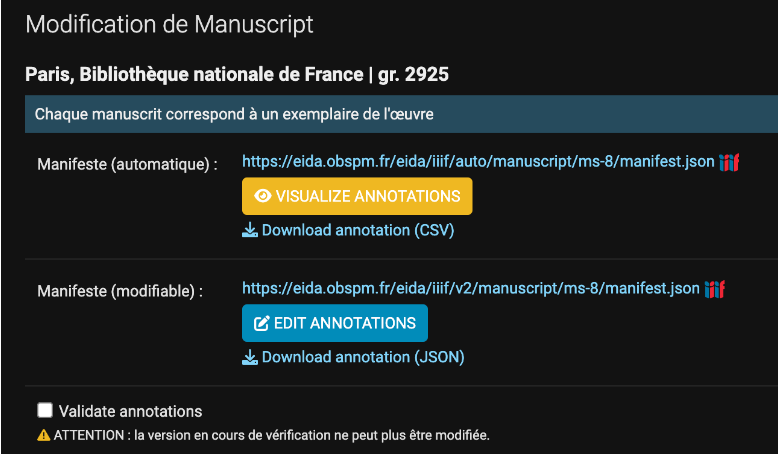
\includegraphics[width=12cm]{images/eida_buttons.png}
		\caption{Capture d'écran des boutons pour la visualisation du document numérisé et l'édition des annotations générées par le modèle de détection}
		\label{fig:eida_buttons}
	\end{figure}
	
	Ainsi, cette chaîne de traitement pour la détection automatique des objets dans les numérisations des sources remplace une recherche manuelle -- par les chercheurs -- des illustrations dans les ouvrages, permettant le traitement d'un corpus plus volumineux en un temps réduit. La détection ne représente cependant qu'une première étape pour le traitement des sources : elle est suivie d'interventions par les chercheurs, qui s'assurent notamment de la pertinence des traitements automatiques effectués.

    \subsubsection{Traitements automatiques, traitements manuels}
   	L'automatisation n'exclut pas un certain nombre d'actions manuelles sur les sources, et l'utilisation d'algorithmes de vision artificielle ne remplace pas le regard critique que peuvent porter les chercheurs sur les sources : il est donc nécessaire, dans les chaînes de traitement définies par les projets, de trouver un équilibre entre étapes automatiques et étapes manuelles de traitement des sources historiques, pour assurer, en finalité, des résultats les plus pertinents possibles.
   	
    Face à ce constat, il est nécessaire, pour les ingénieurs, de concevoir une chaîne de traitement qui va au-delà des étapes automatisées, et qui prend en compte la nécessité d'interventions manuelles entre chaque traitement pour un ajustement des résultats et une analyse primaire des données de sortie. Pour espérer produire des recherches aux résultats pertinents, il est ainsi nécessaire de savoir intégrer l'outil qu'est le \dl à un \textit{workflow}, et de trouver l'équilibre entre automatisation et tâches manuelles.
	
	La chaîne de traitement proposée par \eida propose ainsi une alternance d'étapes automatisées, en bleu sur le schéma, et d'étapes d'analyse par les chercheurs du projet, en violet (fig. \ref{fig:eida_workflow}).
    
    \begin{figure}[h]
    	\centering
    	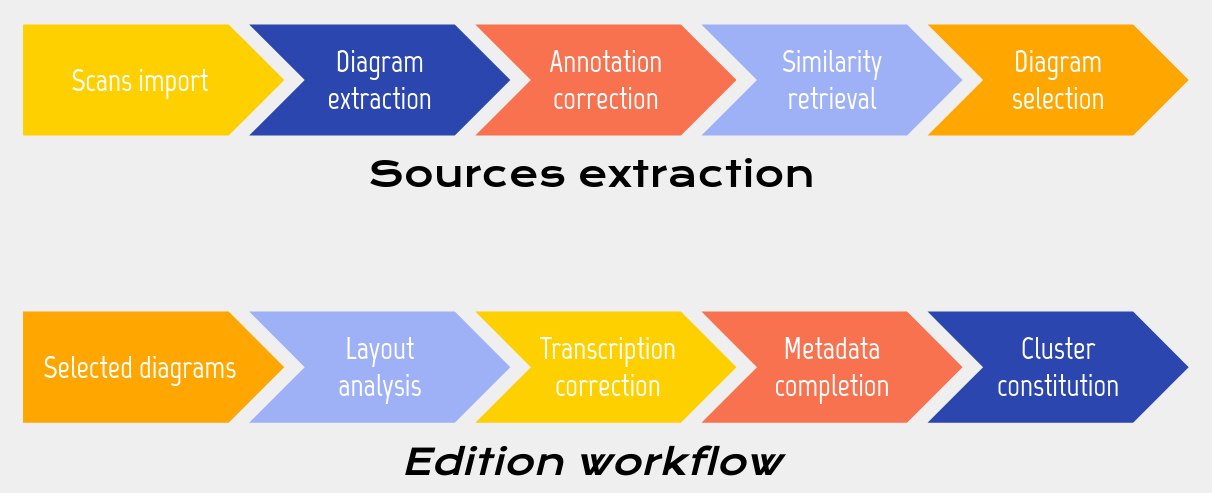
\includegraphics[width=16cm]{images/eida_workflow.png}
    	\caption{Schéma de la chaîne de traitement prévisionnelle des sources du projet \eida}
    	\label{fig:eida_workflow}
    \end{figure}

	Nous constatons ainsi que, suivant ce processus, l'\ia est employée comme un outil de pré-traitement des sources, permettant de naviguer un corpus volumineux et proposer une sélection de sources pour l'analyse par les chercheurs. Cette manière de procéder permet d'exploiter les forces des traitements par algorithmes de vision, et notamment la capacité à traiter un volume de données important en un temps très court. Pour la détection d'objet, la vision artificielle permet d'extraire automatiquement les illustrations d'un manuscrit en quelques minutes : les illustrations extraites devront toujours être corrigées par le chercheur\footnote{Comme expliqué dans le chapitre \ref{objectifsPossibilites}, il est nécessaire pour les performances de l'algorithme d'exclure ou d'inclure un certain nombre de cas limites lors de l'entraînement du modèle, ce qui donne en finalité un modèle de détection qui ne détecte pas nécessairement toutes les illustrations qui pourraient être jugées pertinentes par les chercheurs, ou qui détecte comme d'intérêt des illustrations sans rapport avec le projet de recherche.}, mais cette correction reste moins chronophage qu'une recherche manuelle des illustrations dans chaque source étudiée. L'alternance d'étapes manuelles et d'étapes automatiques permet d'assurer la pertinence des analyses produites, et de contrebalancer certains défauts -- tels que la binarité -- des algorithmes de \cv.
	
	Ainsi, les ingénieurs ont pour rôle -- en dialogue avec les équipes de recherche en histoire et les équipes de recherche en vision artificielle -- l'établissement d'une chaîne de traitement qui exploite les possibilités de la vision artificielle en prenant en compte ses limites. Le \textit{workflow} appliqué doit donc intégrer suffisamment d'étapes de correction manuelle pour produire, en finalité, des résultats pertinents, sans pour autant faire perdre son intérêt à l'usage d'algorithmes de \cv en nécessitant une trop grande intervention des chercheurs. Cet équilibre permet, en finalité, d'assurer la pertinence des données publiées par le projet de recherche, qui auront été étudiées par un prisme critique, tout en exploitant les avantages apportés par l'\ia en termes de volume des corpus traités.
	Ainsi, les ingénieurs ont pour rôle l'établissement d'une chaîne de traitement qui trouve un équilibre entre les possibilités et les limites de la vision artificielle. Le \textit{workflow} appliqué doit donc intégrer suffisamment d'étapes de correction manuelle pour produire, en finalité, des résultats pertinents, sans pour autant faire perdre son intérêt à l'usage d'algorithmes de \cv en nécessitant de trop nombreuses interventions des chercheurs. Cet équilibre permet ainsi, en finalité, d'assurer la pertinence des données produites par le projet de recherche, qui auront été analysées avec un regard critique que seuls les chercheurs peuvent apporter, et auront également bénéficié des avantages de l'\ia en termes de volume des corpus étudiés. 
	
\subsection{Annoter dans une interface graphique}
Pour permettre aux chercheurs des projets \eida et \vhs de corriger les annotations produites par l'algorithme de détection, une interface graphique est développée. En amont de l'entraînement du modèle de détection qui sera utilisé dans la version finale de l'application \eida, ces interfaces pour l'annotation ont pour objectif de fluidifier la constitution de vérités de terrain, c'est-à-dire la production d'un ensemble de numérisations annotées par les chercheurs qui serviront à l'entraînement et à la validation du modèle\footnote{Les données corrigées seront exportées par les ingénieurs des deux projets dans des formats correspondants à ceux attendus pour l'entraînement du modèle, c'est-à-dire images et texte brut.}.
 
Ces interfaces de correction des annotations, intégrées à l'application, rendent accessibles à l'utilisateur les résultats de la détection d'objet effectuée par le modèle de vision, par le biais d'une interface graphique qui lui permet de modifier ces données aisément. Après la mise en place d'un modèle entraîné et le déploiement de l'application, elles permettront aux chercheurs de corriger les annotations faites par le modèle pour en exploiter les résultats pour leurs travaux de recherche.

Les réflexions autour du développement de cette interface s'axent essentiellement autour de la praticité et d'une prise en main aisée, qui permet une correction rapide des résultats de la détection. Le projet \eida a ainsi fait le choix de deux interfaces liées, une première pour la suppression des objets détectés ne correspondant pas aux besoins du projet, et une seconde pour l'ajout d'objets manqués par le modèle et pour la modification des annotations non-conforme aux attentes. L'interface de suppression (fig. \ref{fig:eida_delete_anno}) se présente sous la forme d'une liste d'images des pages de la numérisation, accompagnées d'images des objets détectés, qu'il est possible de supprimer en les sélectionnant puis en cliquant sur un bouton. Cette interface vise à proposer une vue d'ensemble de l'ouvrage numérisé sans nécessiter la consultation de la numérisation en parallèle, pour fluidifier la correction.
 	
 	\begin{figure}[h]
	\centering
	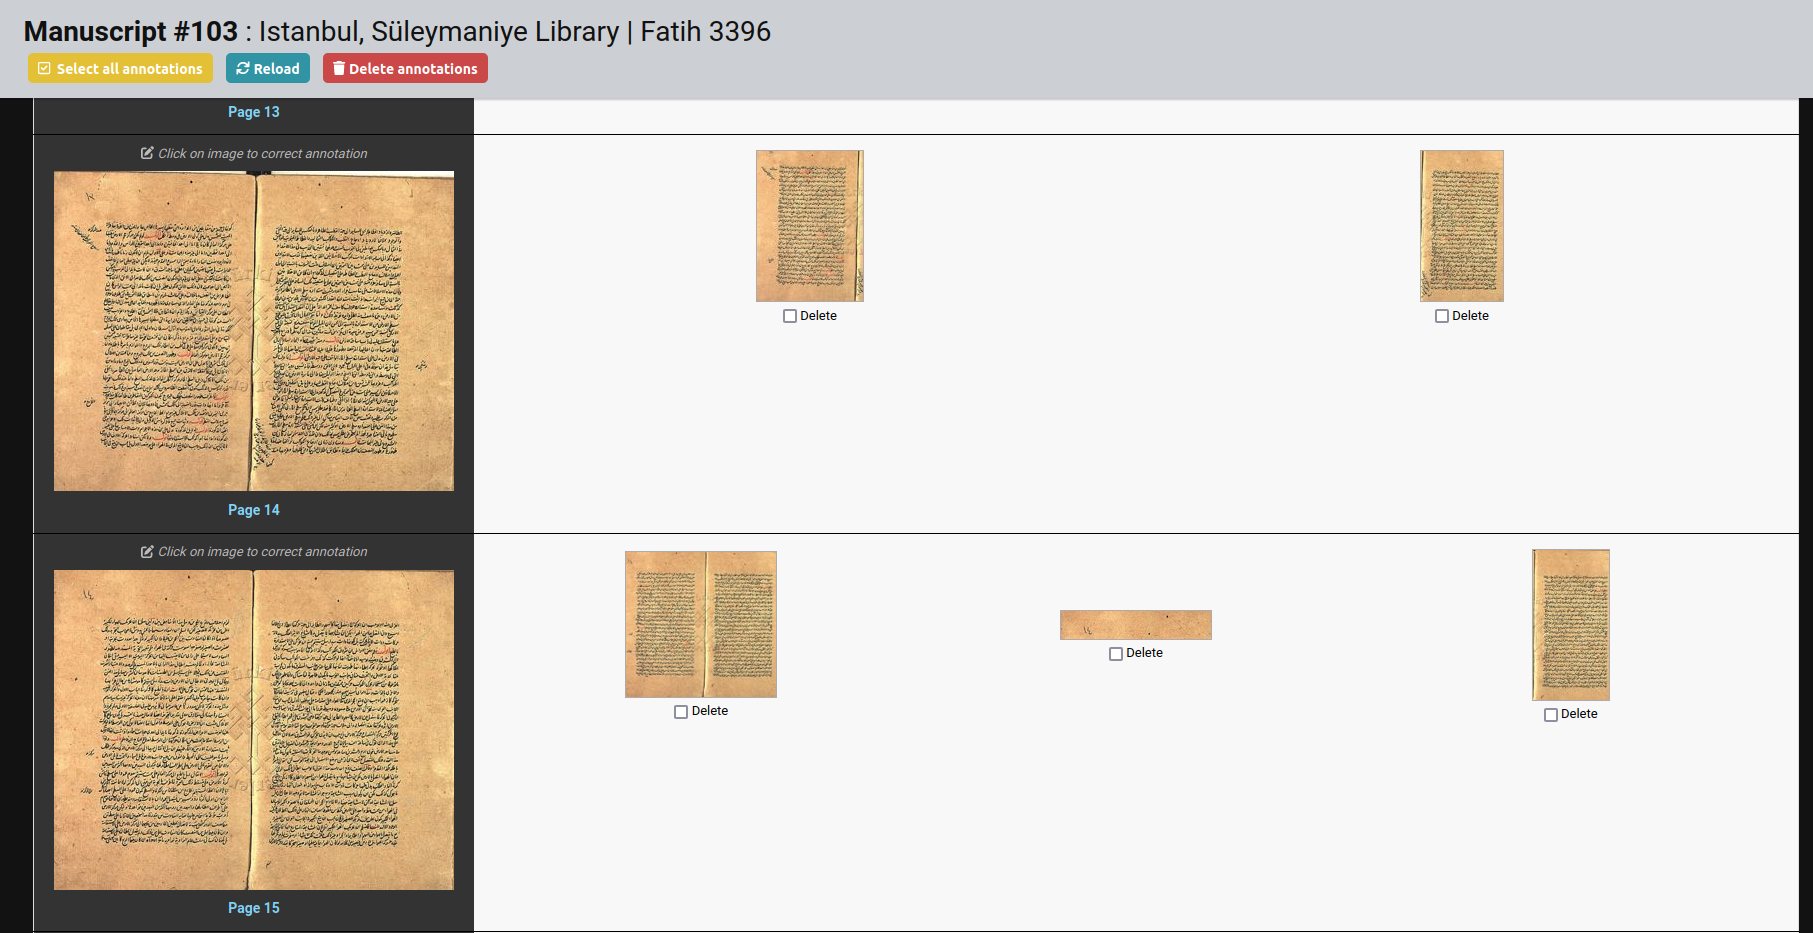
\includegraphics[width=16cm]{images/eida_delete_anno.png}
	\caption{Capture d'écran de l'interface \eida de suppression d'annotations}
	\label{fig:eida_delete_anno}
\end{figure}

Basée sur un visualiseur Mirador\footcite{MiradorHomea}, l'interface d'ajout et de modification des annotations exploite les possibilités offertes par le standard \iiif en intégrant à l'application \eida un outil \textit{open-source} apte à gérer les numérisations et leurs annotations, sans nécessiter de développement spécifique. Par cette interface, les chercheurs ont la possibilité d'ajouter des annotations ou de modifier le format des annotations déjà présentes, pour signaler des illustrations non-détectées ou adapter une détection fautives aux attentes du projet en termes d'annotations.

 	\begin{figure}[h]
	\centering
	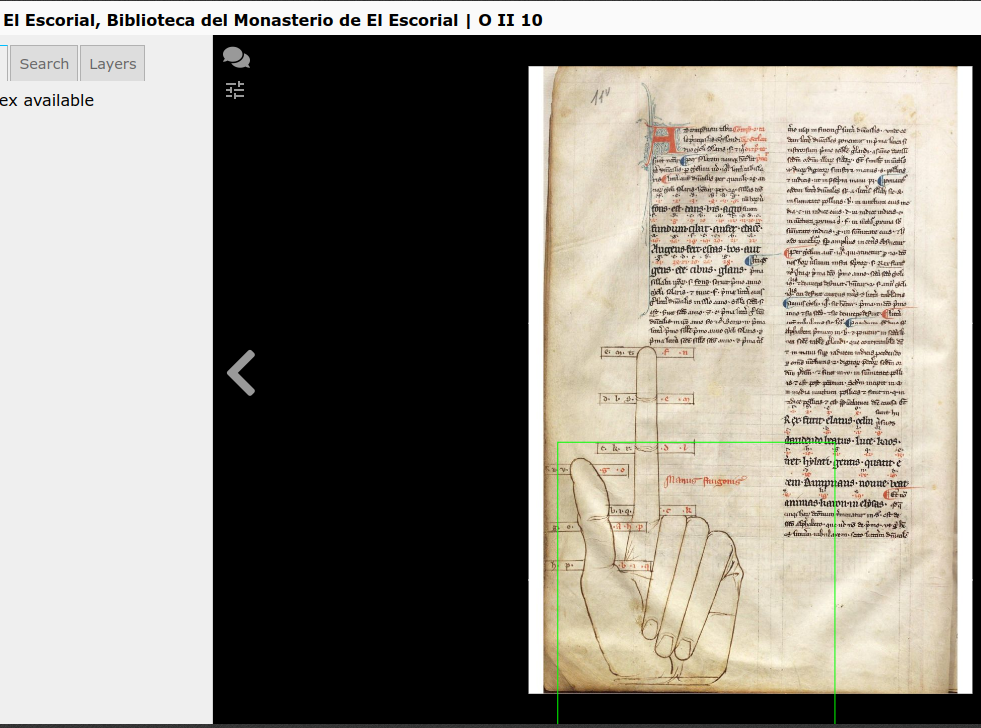
\includegraphics[width=14cm]{images/eida_add_anno.png}
	\caption{Capture d'écran du visualiseur Mirador \eida pour l'ajout et la modification des annotations}
	\label{fig:eida_add_anno}
\end{figure}

L'utilisation d'un visualiseur \iiif pour la gestion des annotations permet, pour les chercheur familiers avec le standard et ses outils, de prendre en main aisément cette interface de correction. Une documentation, rédigée par l'équipe d'ingénierie du projet \eida, est mise à disposition des chercheurs du projet pour la prise en main de ces interfaces : cette documentation permet d'assurer l'établissement d'une norme dans les choix effectués en termes de correction des données pour l'entraînement du modèle. Dans le futur, en prévision de la publication de l'application, une documentation destinée au grand public est à envisager, axée sur la prise en main des interfaces pour la correction de l'annotation par le modèle, sans l'enjeu de l'uniformisation des données pour l'entraînement. Une distinction est à faire entre les besoins actuels qui entourent ces interfaces, axés autour de l'entraînement de modèles de détection encore généralistes, et les besoins futurs, dans une application publiée et accessible à tous, où ces interfaces serviront à une correction en autonomie par les utilisateurs.
